\documentclass[11pt]{article}
\usepackage{graphicx}
\usepackage{float}
\usepackage{caption}


% *********  Set some sensible page margins  ***********
\setlength{\oddsidemargin}{0in} \setlength{\evensidemargin}{0in}
\setlength{\textwidth}{6.2in}
\setlength{\topmargin}{-1in} \setlength{\textheight}{9.8in}

\title{Mounting M: drive in the Orchard on OS X}
\author{Daniel K Monaghan (dkm2@aber.ac.uk)}
\date{December 2014}

\begin{document}
\maketitle


\begin{figure}[H]
    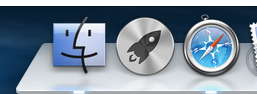
\includegraphics[width=0.5\textwidth]{images/mdrive-1.png}
    \caption*{1. Open \textbf{Finder} by clicking on its icon on the far left of the Dock, at the bottom of the screen}
\end{figure}

\begin{figure}[H]
    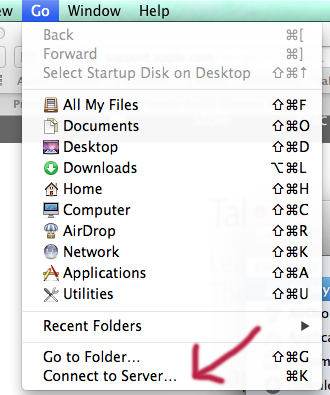
\includegraphics[width=0.5\textwidth]{images/mdrive-2.png}
    \caption*{2. Open the \textbf{Go} menu at the top of the screen, and click \textbf{Connect to Server}}
\end{figure}

\begin{figure}[H]
    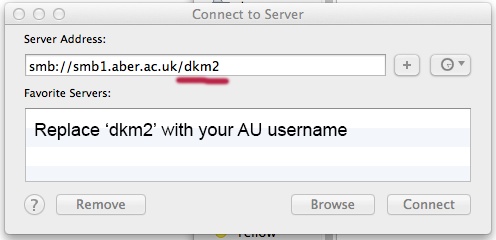
\includegraphics[width=0.5\textwidth]{images/mdrive-3.png}
    \caption*{3. Enter \texttt{smb://smb1.aber.ac.uk/\textbf{your\_username}} and click \textbf{Connect}. The contents of your \texttt{"M:"} drive should then appear}
\end{figure}

\begin{figure}[H]
    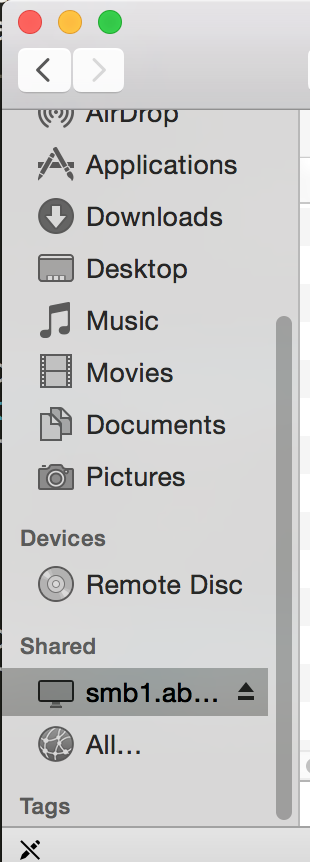
\includegraphics[width=0.25\textwidth]{images/mdrive-4.png}
    \caption*{4. To access your directory later on, open Finder again and look for \texttt{"smb1.aber.ac.uk"} in the sidebar}
\end{figure}


\end{document}
